\clearpage
\section{Versuchsbeschreibung}
\subsection{Verwendete radioaktive Proben}
\subsubsection{Natrium}
In diesem Versuch wird das Natrium-Präparat $^{22}Na$ verwendet. Bei diesem tritt $\beta$-, aber kein $\alpha$-Zerfall auf. Dabei handelt es sich in etwa 89,9 \% der Fälle um $\beta^{+}$-Zerfall, in den restlichen 10,1 \% kommt es zu Elektroneneinfang. Die Zerfallsgleichungen sehen dabei folgendermaßen aus:\\
\textbf{$\beta^{+}$-Zerfall}: \[^{22}_{11}Na\rightarrow ^{22}_{10}Ne+e^{+}+\nu_{e}.\]
\textbf{Elektroneneinfang}:
\[^{22}_{11}Na+e^{-}\rightarrow ^{22}_{10}Ne+\nu_{e}.\]
Die für die Energieeichung verwendeten charakteristischen Spektrallinien liegen bei 0,511 MeV und 1,274 MeV (Quelle: [sta]).
\subsubsection{Cobalt}
Es wird $^{60}_{27}Co$ verwendet. Dabei kommt es so gut wie ausschließlich zu \textbf{$\beta^{-}$-Zerfall}: \[^{60}_{27}Co\rightarrow ^{60}_{28}Ni+e^{-}+\overline{\nu_{e}}.\] Die charakteristischen Spektrallinien liegen bei 1,173 MeV und 1,333 MeV (Quelle: [sta]).
\subsubsection{Europium}
Bei Europium kommt es zu allen drei Arten von $\beta$-Zerfall:\\
\textbf{$\beta^{-}$-Zerfall} \[^{152}_{63}Eu\rightarrow ^{152}_{64}Gd+e^{-}+\overline{\nu_{e}},\]
\textbf{$\beta^{+}$-Zerfall}
\[^{152}_{63}Eu\rightarrow ^{152}_{62}Sm+e^{+}+\nu_{e},\]
\textbf{Elektroneneinfang} \[^{152}_{63}Eu+e^{-}\rightarrow ^{152}_{62}Sm+\nu_{e}.\]
Das Spektrum von Europium weist mehrere charakteristische Spektrallinien auf. Zur Energieeichung werden die beiden intensivsten Linien mit Energien von 0,122 MeV bzw. 0,344 MeV (Quelle: [sta]) verwendet.
\clearpage
\subsubsection{Thorium}
$^{228}Th$ zerfällt unter $\alpha$ und $beta$-Zerfall. Die Zerfallskette sieht folgendermaßen aus: 
\begin{figure}[h]
\begin{center}
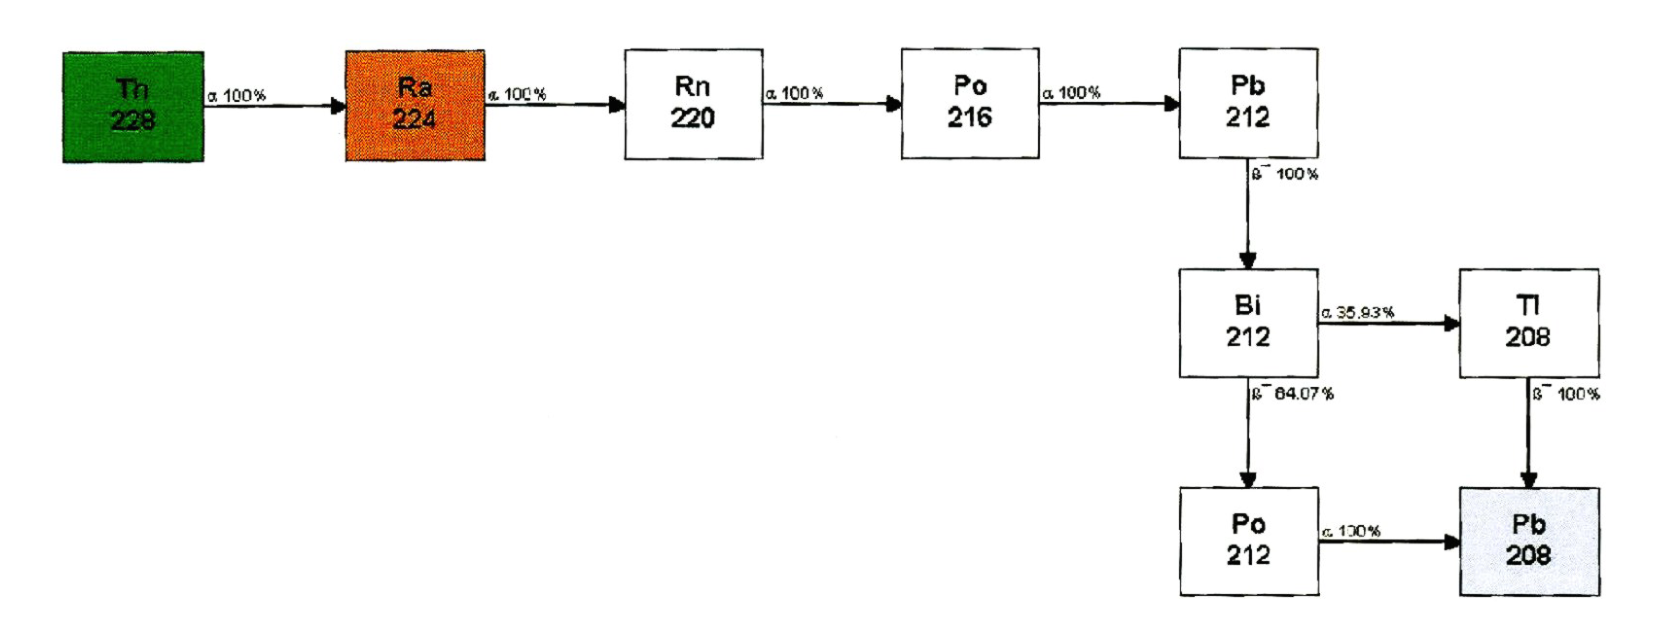
\includegraphics[scale=0.3]{Bilder/zerfall}
\caption{Zerfallskette von $^{228}Th$ (Quelle: [ver].)}
\end{center}
\end{figure}
Die Energien der mit den Übergängen verbundenen emittierten $\gamma$-Strahlung werden in der Auswertung dem aufgenommenen Spektrum zugeordnet.

\subsection{Aufbau und Durchführung}
Der Versuch besteht aus zwei Szintillationszählern (NaJ und Plastik), welche beide auf die Haltevorrichtung der Probe gerichtet sind. Beide besitzen einen eingebauten Vorverstärker welche auf Grund dessen nicht im unten folgenden Schaltbild aufgeführt sind. Dabei wird der registrierte Ladungspuls über einen Kondensator entladen und die an einem bekannten Widerstand abfallende Spannung gemessen. Das hierbei entstehende Signal wurde skizziert und dem Anhang beigefügt.\\
Dieses Signal wurde anschließend durch den Main Amplifier (MA) weiter verstärkt und in ein für den Multi-Channel-Analyser (MCA) messbaren Puls umgewandelt. Der MA hat zwei verschiedene Ausgänge, einen uni- und ein bi-polarer Ausgang. Auch von diesen Ausgängen wurde jeweils eine Skizze angefertigt und kann im Anhang betrachtet werden. Durch diese Ausgänge lässt sich auch die Verzögerung durch die Elektronik messen.\\
\begin{figure}[h]
\begin{center}
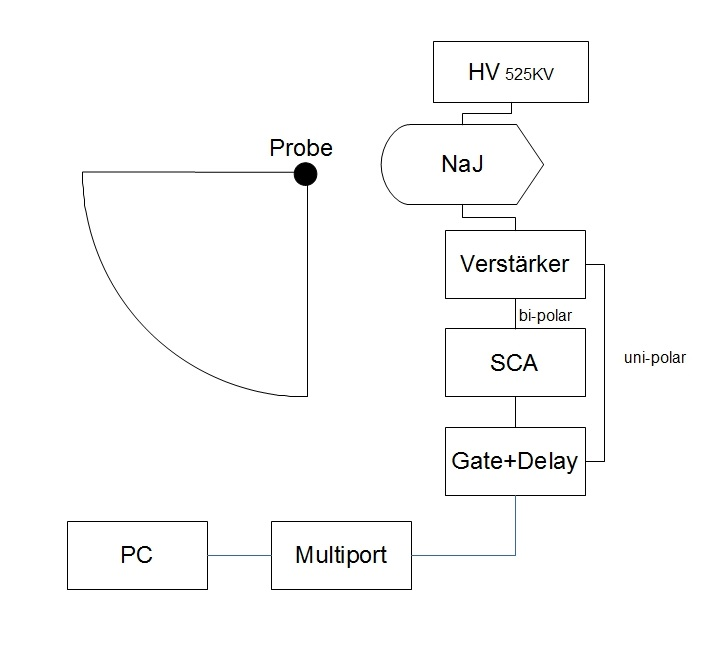
\includegraphics[scale=0.35]{aufbau1}
\caption{Aufbau zur Messung der Spektren.}
\label{fig:aufbau1}
\end{center}
\end{figure}
Zur Messung der Spektren wird das unipolare Signal in de MCA gegeben. Dieser ordnet die Energie (Pulshöhe) der gemessenen Pulse in eine Kanalnummer um und leitet die Information an den Computer weiter. Dort wird ein Histogramm über die einzelnen Kanäle des MCA aufgenommen. Durch eine im Durchgeführte Energieeichung kann die Energie der einzelnen Kanäle bestimmt werden. Auf diese Weise wurden die Spektren von Natrium, Cobalt, Europium und Thorium, sowie der Untergrund aufgenommen. Die Schaltung für diese Messungen sind im oben gezeigten Schaltbild gegeben (Abb \ref{fig:aufbau1}).
Für die Messung der Koinzidenzmessungen sind  zusätzliche geräte zur Signalverarbeitung nötig. Es wird für jeden Szintillator ein Single-Channel-Analyser (SCA) verwendet um ausschließlich die aus der Paarbildung resultierenden $\gamma$-Quanten der Energie 0,511 MeV zu registrieren. In diesen SCA lassen sich eine untere und eine obere Grenze für die Energie der durchgelassenen Pulse festlegen. Diese Pulse werden dann in ein einheitliche Rechteckpulse umgewandelt. Die Information über die Pulshöhe geht dabei verloren. Da bei dieser Umwandlung eine geringe Zeitabweichung deutlich wichtiger ist als eine genaue Energie, wird der bipolare Ausgang des MA in den SCA geleitet. Der Spannungsverlauf kann wieder dem Anhang entnommen werden. Das Signal des Plastikszintillators muss zusätzlich noch durch ein Delay verzögert werden, damit man die Rechtecksignale der beiden Szintillatoren auf Koinzidenzen überprüfen kann, da dieses Signal deutlich früher eintrifft. Zur Messung der Koinzidenzen werden beide Signale in die Timing-Unit gegeben. Diese gibt für zwei gleichzeitig ankommende Signale einen Count auf dem angeschlossenen Zähler. Das Delay zwischen den Szintillatoren muss dabei entsprechend so eingestellt werden, dass die Timing-Unit jede Koinzidenz als solche erkennt. Diese Einstellung konnte mithilfe des Oszilloskops durchgeführt werden.\\
Der Aufbau ist auch noch einmal im folgenden Abbildung \ref{fig:aufbau2} illustriert.
\begin{figure}[h]
\begin{center}
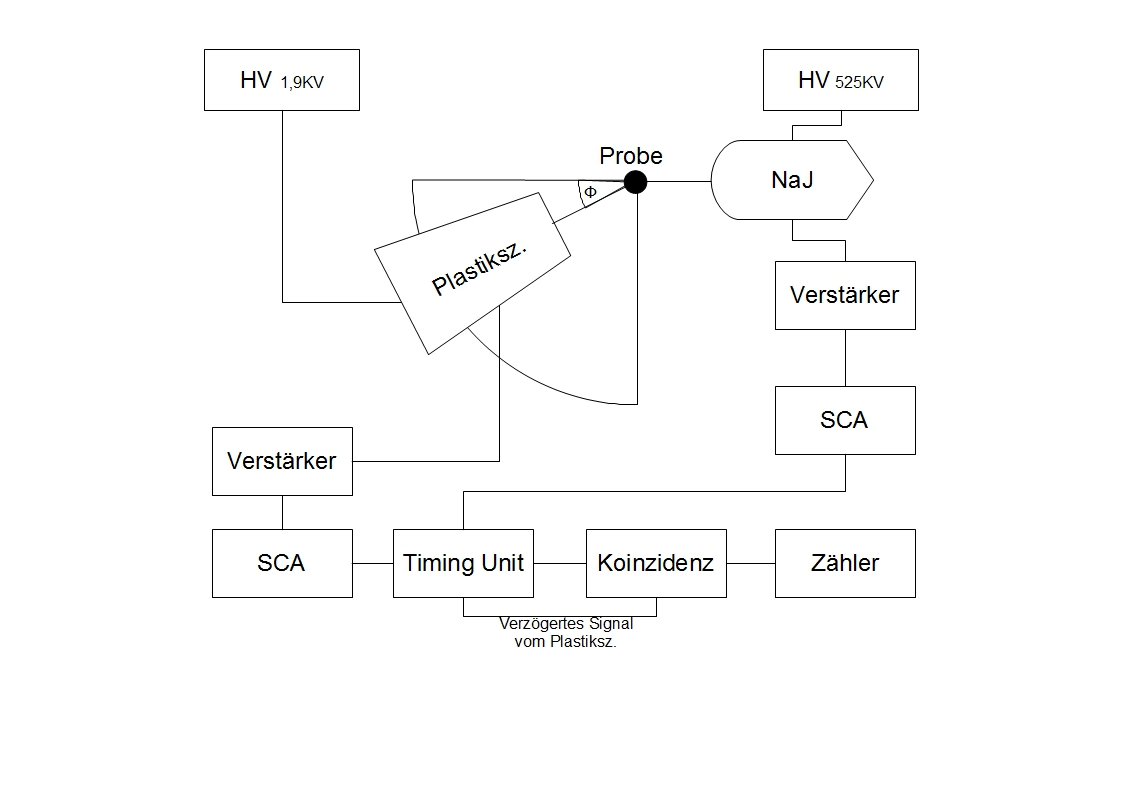
\includegraphics[scale=0.4]{aufbau2}
\caption{Aufbau zur Messung der Koinzidenzen.}
\label{fig:aufbau2}
\end{center}
\end{figure}